\section{Results} \label{sec:results}

\section{Convergence results}\index{convergence results!INS}

This section details the results of various convergence tests. 
Convergence results are run using the {\bf twilight-zone} option, also
known less formally as the {\bf method of analytic solutions}.
In this case the equations are forced so the the solution will
be a known analytic function.

The tables show the maximum errors in the solution components. The rate shown is estimated convergence rate, $\sigma$,
assuming ${\rm error} \propto h^\sigma$. The rate is estimated by a least squares fit to the data.

The 2D trigonometric solution used as a twilight zone function is
\begin{align*}
    u &= \half \cos(\pi \omega_0 x) \cos(\pi \omega_1 y) \cos( \omega_3 \pi t) + \half\\
    v &= \half \sin(\pi \omega_0 x) \sin(\pi \omega_1 y) \cos( \omega_3 \pi t) + \half\\
    p &=       \cos(\pi \omega_0 x) \cos(\pi \omega_1 y) \cos( \omega_3 \pi t)  + \half
\end{align*}
The 3D trigonometric solution is
\begin{align*}
    u &=       \cos(\pi \omega_0 x) \cos(\pi \omega_1 y) \cos(\pi \omega_2 z) \cos( \omega_3 \pi t) \\
    v &= \half \sin(\pi \omega_0 x) \sin(\pi \omega_1 y) \cos(\pi \omega_2 z) \cos( \omega_3 \pi t) \\
    w &= \half \sin(\pi \omega_0 x) \sin(\pi \omega_1 y) \sin(\pi \omega_2 z) \cos( \omega_3 \pi t) \\
    p &= \half \sin(\pi \omega_0 x) \cos(\pi \omega_1 y) \cos(\pi \omega_2 z) \sin( \omega_3 \pi t) 
\end{align*}
When $\omega_0=\omega_1=\omega_2$ it follows that $\grad\cdot\uv=0$.
There are also algebraic polynomial solutions of different orders.


\begin{table}[hbt]
\begin{center}
\begin{tabular}{|l|c|c|c|c|c|c|c|} \hline
grid        & N      &  p      &  u       & v        &  T       & $\grad\cdot\uv$  &  $T_s$            \\ \hline 
innerOuter1 &  20    & 1.32e-02 &  3.69e-03 &  2.74e-03 &  8.37e-04 &  2.68e-02   &    1.75e-03 \\
innerOuter2 &  40    & 2.17e-03 &  4.03e-04 &  3.26e-04 &  1.85e-04 &  5.01e-03   &    4.33e-04\\
innerOuter4 &  80    & 4.20e-04 &  5.31e-05 &  3.89e-05 &  4.55e-05 &  1.71e-03   &    1.09e-04\\\hline 
\end{tabular}
\caption{Inner-outer. Maximum errors, polynomial, $t=1.$, $\nu=.1$, $k_T=\nu/P_r$, $k_s=.01$ (?).}
\label{table:innerOuterTZ}
\end{center}
\end{table}


\begin{figure}
\begin{center}
  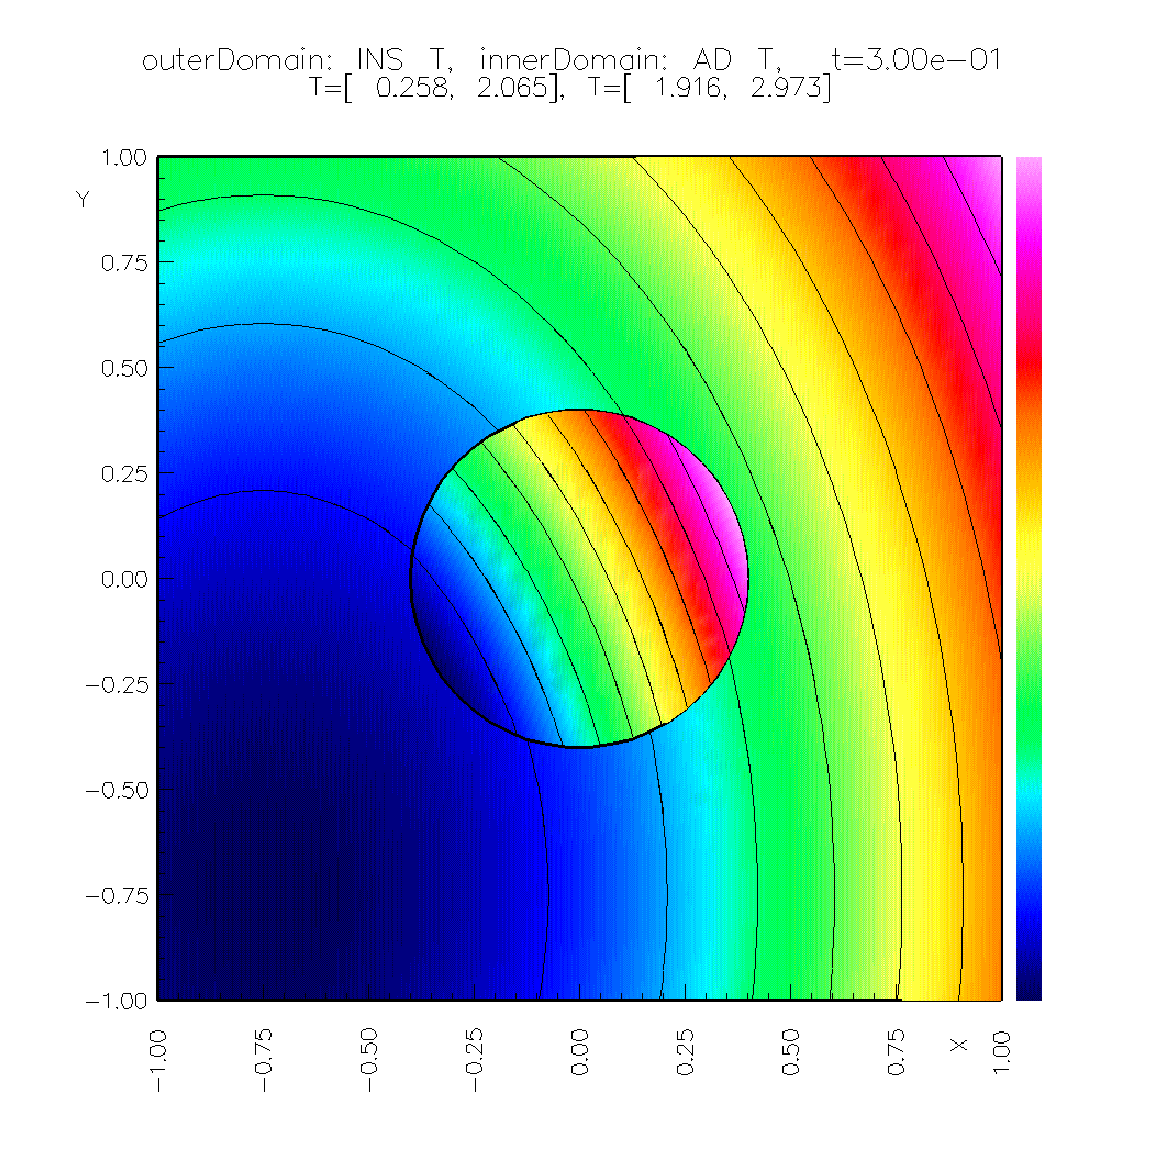
\includegraphics[width=4.0in]{innerOuterINS.AD.TZ.ps}
\end{center}
\caption{INS outside, AD inside, TZ.}
\label{fig:innerOuterTZ}
\end{figure}

\bogus{


cgmp io.cmd -g="innerOuter2d.hdf" -tz=1 -solver=yale -tp=1
============= Cgins time-step info for domain 0 (outerDomain)(fluid) steps=410==================
     t    err(p)   err(u)   err(v)   err(T)    div       uMax     dt       cpu
   1.000 1.32e-02 3.69e-03 2.74e-03 8.37e-04 2.68e-02  7.33e+00 2.45e-03 7.54e+00
============= Cgad time-step info for domain 1 (innerDomain)(solid) steps=410==================
     t    err(T)    uMax     dt       cpu    mem (Gb)
   1.000 1.75e-03 4.62e+00 2.18e-02 7.54e+00        0

innerOuter2d2.hdf
============= Cgins time-step info for domain 0 (outerDomain)(fluid) steps=1644==================
   1.000 2.17e-03 4.03e-04 3.26e-04 1.85e-04 5.01e-03  7.33e+00 6.09e-04 3.62e+01
============= Cgad time-step info for domain 1 (innerDomain)(solid) steps=1644==================
   1.000 4.33e-04 4.62e+00 7.61e-03 3.62e+01        0

innerOuter2d4.hdf
============= Cgins time-step info for domain 0 (outerDomain)(fluid) steps=6547==================
   1.000 4.20e-04 5.31e-05 3.89e-05 4.55e-05 1.71e-03  7.33e+00 1.53e-04 3.52e+02
============= Cgad time-step info for domain 1 (innerDomain)(solid) steps=6547==================
   1.000 1.09e-04 4.62e+00 2.13e-03 3.52e+02        0

} % end bogus




% Tables~(\ref{table:ins.square}-\ref{table:ins.box}) show results from running Cgins on various
% grids. 

% \input \convDir/ins.square.order2.table.tex
% \input \convDir/ins.square.order4.table.tex
% \input \convDir/ins.cic.order2.table.tex
% \input \convDir/ins.cic.order4.table.tex
% \input \convDir/ins.box.order2.table.tex
% \input \convDir/ins.box.order4.table.tex
% \input \convDir/ins.sib.order2.table.tex
% \input \convDir/ins.sib.order4.table.tex
% 
% \begin{figure}[htb]
%   \begin{center}
%    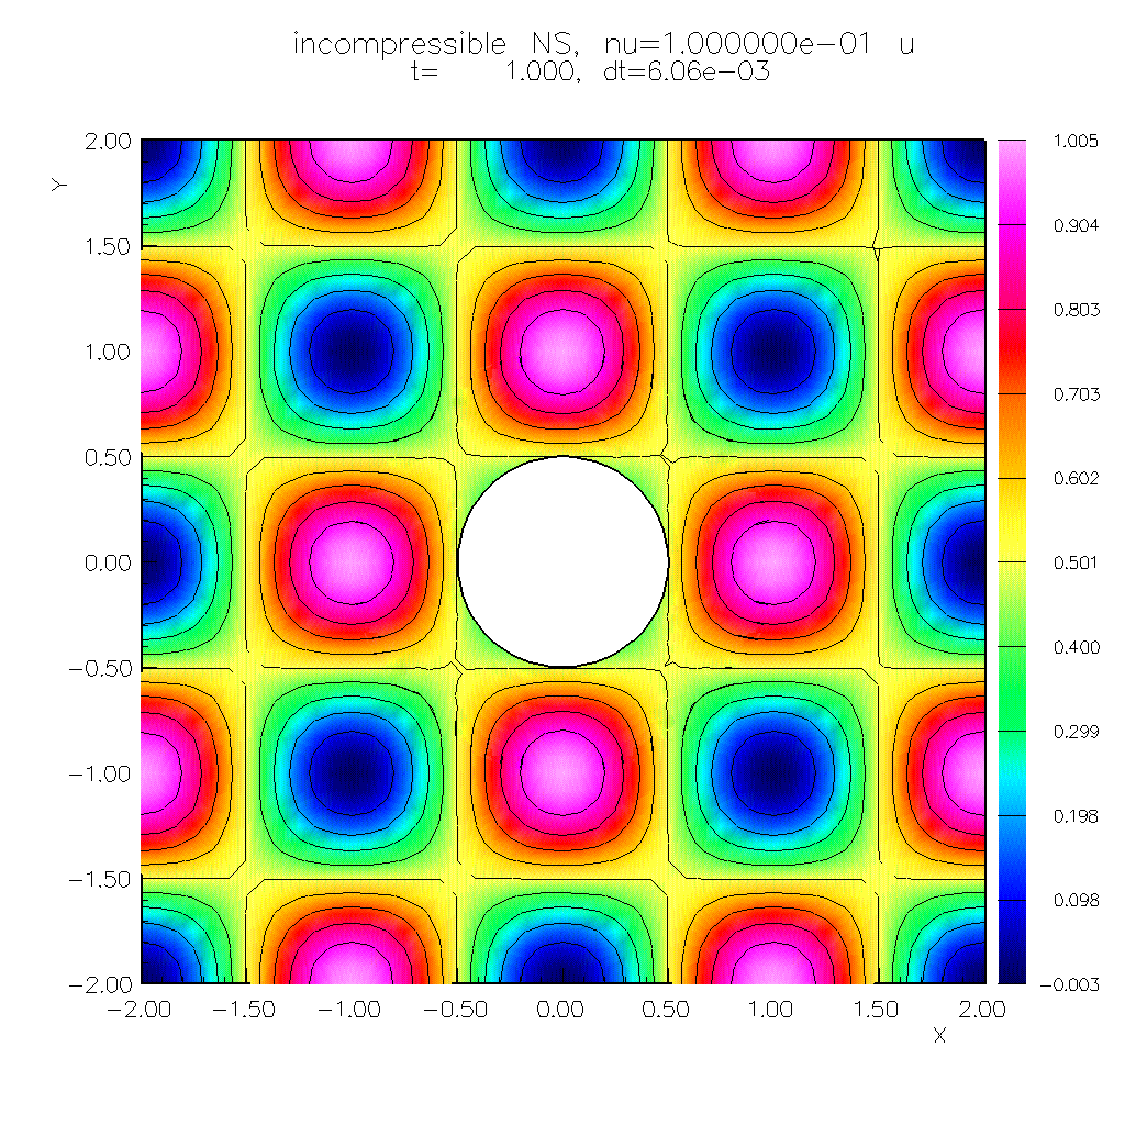
\epsfig{file=\obFigures/ins.cic3.tz.ps,width=.7\linewidth} 
%   \caption{Incompressible N-S, twilight zone solution for convergence test} \label{fig:ins.cic.tz}
%   \end{center}
% \end{figure}
